\chapter{User Documentation}
\label{user}
This software intends to demonstrate the user how our domain specific language works to manipulate the global stack. In this chapter, the application will be explained from an end-user perspective with demonstration on how to build and run the program and how to enter input-output pairs to get the program that achieve a certain function.

\section{Main Methods and Tools}
\label{sec:tools}
The user interface is written using PySimpleGUI \cite{psgui}, a Python package that enables Python programmers of all levels to create GUIs. PySimpleGUI is currently capable of running on 4 Python GUI Frameworks, they are PySimpleGUI, PySimpleGUIQt, PySimpleGUIWx, and PySimpleGUIWeb. Here we used the default PySimpleGUI Framework. The algorithm that implements the DSL and builds the model is written in Python 3. We used the typing module which was introduced in Python 3.5 \cite{typing} to do the type check and the package PyTorch \cite{pytorch} to build the neural nets.

\section{Installing}
\label{install}
The installation of the software is relatively straightforward and simple. This section will walk the end-user through the process of setting up the environment, installing dependencies, and running the program.

\subsection{Environment}
The development environment is typically a workstation for developers, while the production environment is a real-time setting where programs are run and used by end users. In this project, we will implement the app and run the tests in the development environment.

The specification of the system used to develop this application consists of:
\begin{itemize}
    \item Operating System: macOS Big Sur
    \item Ram: 16.0 GB
    \item CPU: 2.0 GHz
    \item Code Editor: Visual Studio Code
    \item Python 3.8.0 ( requirement: Python 3.5, 3.6, 3.7, 3.8)
\end{itemize}
\subsection{Installation}
We have all the prerequisites written in requirements.txt and environment.yml, you can built dependencies easily with those files in either of the following methods.
\noindent Method 1: If you have \texttt{Python}, \texttt{pip} installed, you can use the following steps:
\begin{enumerate}
	\item 	Open a terminal and change to the project directory.
	\begin{itemize}
		\item Install virtualenv: \texttt{pip install virtualenv}
		\item Create a virtual environment: \texttt{virtualenv venv} 
		\item Activate it: \texttt{source venv/bin/activate}
	\end{itemize}
	
	\item Install the requirements: 
	\texttt{pip install -r requirements.txt}
	
	\item Run the app:
	\texttt{python main.py}
	
\end{enumerate}

\noindent Method 2: If you have \texttt{conda} installed, you can follow the steps below to install the dependencies before running the program:
\begin{enumerate}
	\item Open a terminal and change to the project directory.
	\begin{itemize}
	    \item 	Create an environment: 
	    \texttt{conda env create -f environment.yml}
    	\item Activate the environment:
    	\texttt{conda activate stack-prog-synth}
	\end{itemize}

	\item Run the app:
	\texttt{python main.py} 
	
\end{enumerate}

\section{Domain Specific Language}
\label{sec:dsl}
A domain-specific language (DSL) is a small, usually declarative, language that offers expressive power focused on a particular problem domain \cite{dsl}. For the task of program synthesis, the choice of DSL is important. It should be expressive enough to capture the problems that we wish to solve, but restricted as much as possible to limit the difficulty of the search \cite{deepc}. Specifically to our project, the DSL needs to be linear so as to cooperate with the beam search algorithm.

Following this observation, we decided to construct our own DSL in order to restrict search space and simplify the synthesis process. 

Our DSL is a stack-based concatenative language, this section will introduce you the concept of stacks, stack-based programming languages, concatenative, and the advantages of our DSL and the description of its commands. 

\subsection{Stack-based language}
\label{sec:stack-based}
To understand stack-based language, we first need to understand the concept of a stack.

The stack is called that way because it resembles a stack in real life. Like a stack of plates, adding or removing is only possible at the top. They are two main principal operations of a stack as an abstract data type:
\begin{itemize}
    \item Push: adds a new element to the top of the stack.
    \item Pop: removes the top element from the stack.
\end{itemize}

A stack based language works by having a global stack that the code implicitly works with. This means that you don't pass parameters when you call functions: all functions work by pushing and popping onto the global stack. Languages like Factor \cite{factorlan}, Forth, Joy \cite{von2001joy} fit this description.

Here comes an example for stack-based algorithms. Using reverse Polish notation \cite{RPN}, we get the result of the mathematical expression $(16 * 10 + 8)$ this way:

You would write $16 \ 10 * 8 \ +$, and the computer will evaluate from left to right. A value will be pushed onto the stack, a word will be called, assuming the leftmost is the top of the stack. The stack will change as the following when the program is running.

\begin{DispWithArrows*}[fleqn, mathindent = 2cm]
    &<> \Arrow{Push 16 to the stack.} \\
    &<16>\\
    &<10, 16> \Arrow[tikz={text width=10cm}]{The word * takes the top two numbers from the stack, multiplies them, and pushes the product back on the stack.} \\
    &<160>\\
    &<8, 160> \Arrow{The word + adds the top two values, pushing the sum.} \\
    &<168>
\end{DispWithArrows*}

\subsection{Concatenative and stack languages}
Even though the terms stack language and concatenative language sometimes get thrown around interchangeably, they actually represent similar but distinct classes of languages \cite{concat}.

``Concat is a functional language (no explicit
states) with static types and type inference. A
concatenative language can also be dynamically
typed and work without type inference; some variants are also functionally impure.'' \cite{herzberg2009concatenative} Concatenative languages are where the main way to build programs is by composing functions which all manipulate a single object. While stack-oriented languages operate on one or more stacks. They consider data of each stack, by utilising one piece of data from atop the stack, and returning data back atop the stack. 

\subsection{Stack-based concatenative language}
\label{sec:stack-based catlang}
Our DSL was largely inspired by Cat programming language \cite{cat} which is a statically typed stack-based pure functional language. A program in our DSL is a sequence of terms, where each term can change the state of the global stack. 

The figure below shows the syntax of the stack-based concatenative language. The Instruction enclosed in square brackets represents a quotation. A value can be either an integer or a quotation and a term is either a value or an instruction. A program consists of terms which are used to operate the stack. See Section \ref{sec:lang} for a detailed explanation for each instruction.
\begin{figure}[H]
    \centering
    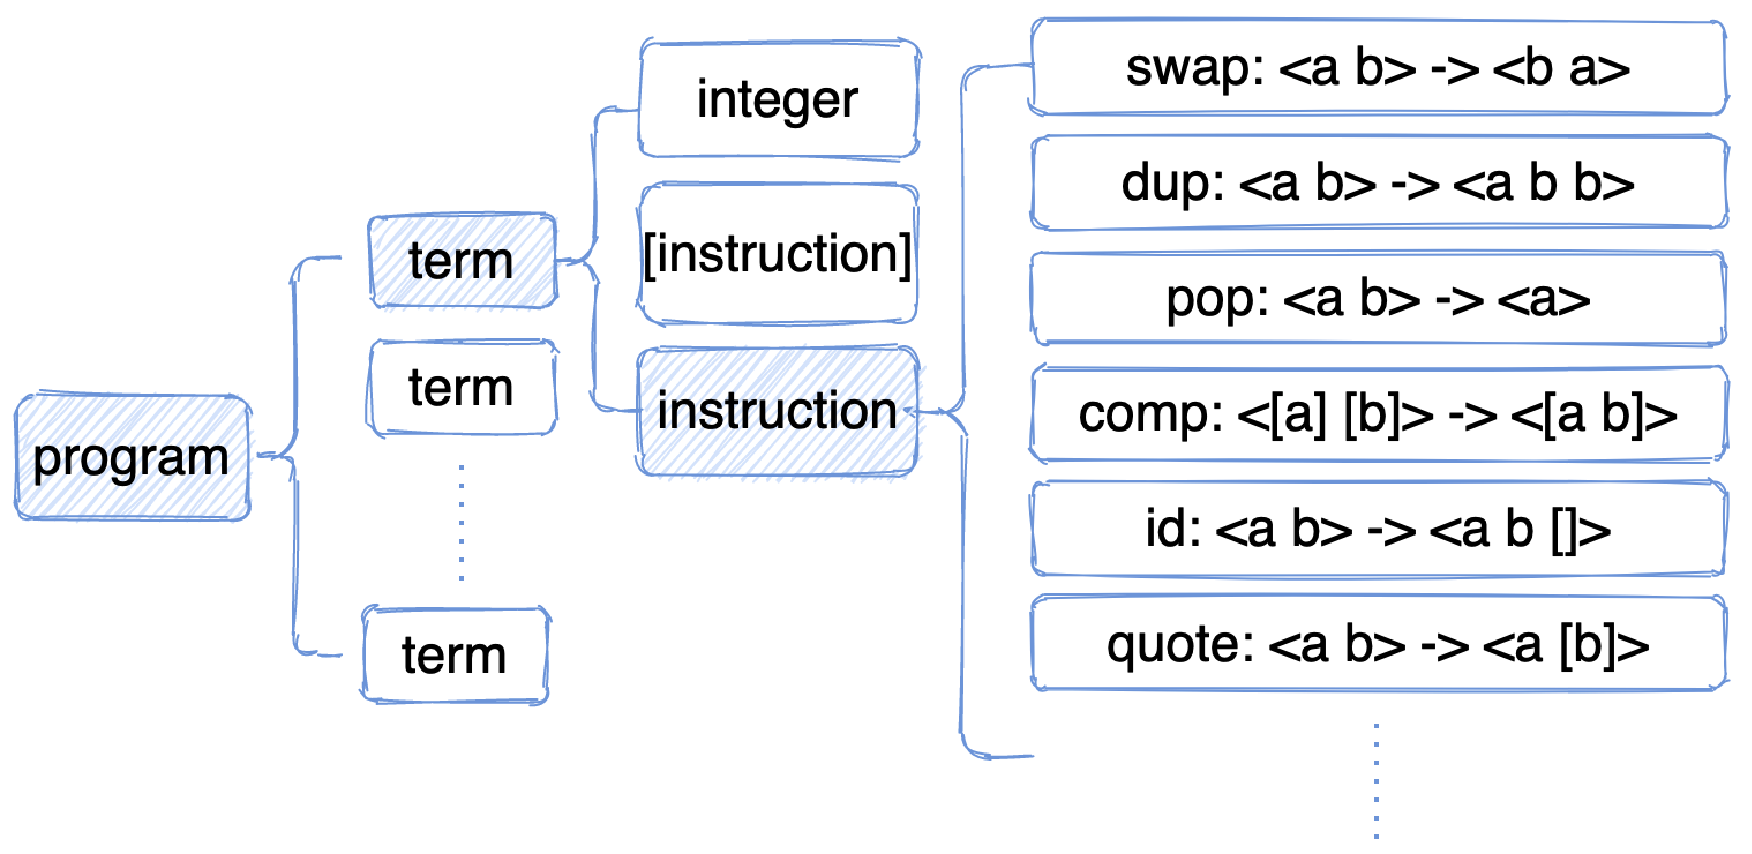
\includegraphics[width=0.8\textwidth]{syntax.pdf}
    \caption{Syntax}
    \label{fig:syntax}
\end{figure}

There are many advantages of our language. Firstly, it is statically typed which means it is easy to filter out bad programs. Secondly, it does not have variables, there is only a list of operations where every operation can manipulate the global stack. Each operation is either a command or a value. All commands in this DSL are functions that take a stack as input, and return a new stack as output. This feature makes the language easy to be generated and encoded, this serves as a great advantage regarding the program synthesis task. Due to the linearity of this language, it is easier to use beam search on it than on other languages. Lastly, in support of higher-order functions, we have a special expression form - quotation. It is a unary constructor, an instruction can be turned into a value by quoting, then it can be pushed into the global stack and applied later. In our DSL the quotation of a program is written by enclosing it in square brackets.

Here is an example: given input stack $<3,5,1>$ and program $[swap, pop, mul]$, assuming the leftmost is the top of the stack. 
\begin{DispWithArrows*}
    &<3, 5, 1> \Arrow{Swap} \\
    &<5, 3, 1> \Arrow{Pop} \\
    &<3, 1> \Arrow{Dup} \\
    &<3, 3, 1> \Arrow{Mul}\\
    &<9, 1> 
\end{DispWithArrows*}

In the end, we have 9, 1 in the resulting stack.

\subsection{Descriptions of stack-based concatenative language}
\label{sec:lang}
During the animated demonstration, you may encounter the following instructions, below are some detailed explanations. 
\begin{description}[labelwidth = 3em, leftmargin = !]
    \item[Swap] For a stack with at least two items, interchange the top two elements.
    \item[Dup] For a stack with at least one item, duplicate the topmost element on the stack.
    \item[Pop] For a stack with at least one item, remove the topmost element from the stack.
    \item[Comp] For a stack with two quoted programs on the top, replace them with a new quotation that is the result of composing the top quotation with the second quotation.
    \item[Id] For any stack, push a quoted identity program to the stack.
    \item[Quote] For a stack with at least one item, turn an integer or an instruction to quotation form. 
    \item[Apply] For a stack with at least one quotation, apply takes the top quoted program, and applies it to the rest of the stack.
    \item[Dip] For a stack with at least one quotation, apply the quoted program under the top most element to the rest of the stack.
    \item[Add] For a stack with at least two integers, add the top two integers.
    \item[Sub] For a stack with at least two integers, subtract the Second integer from the first integer.
    \item[Mul] For a stack with at least two integers, multiply the top two integers.
    \item[Div] For a stack with at least two integers, divide the Second integer with the first integer.
    \item[Mod] For a stack with at least two integers, get the remainder of the second integer divided by the first integer.
\end{description}

\noindent Overall, our DSL contains:
\begin{itemize}
    \item First-order instructions Swap, Dup, Pop, Comp, Id, Quote, Apply, Dip.
    \item Integer instructions Add, Sub, Mul, Div, Mod.
\end{itemize}
By converting them into quotation form, we can use them as higher-order commands.


\section{Using}
\label{using}
\subsection{System functions}

After successfully running the program, you will see the following main screen. It has a brief description of the software and some instructions to the user.
\begin{figure}[H]
    \centering
    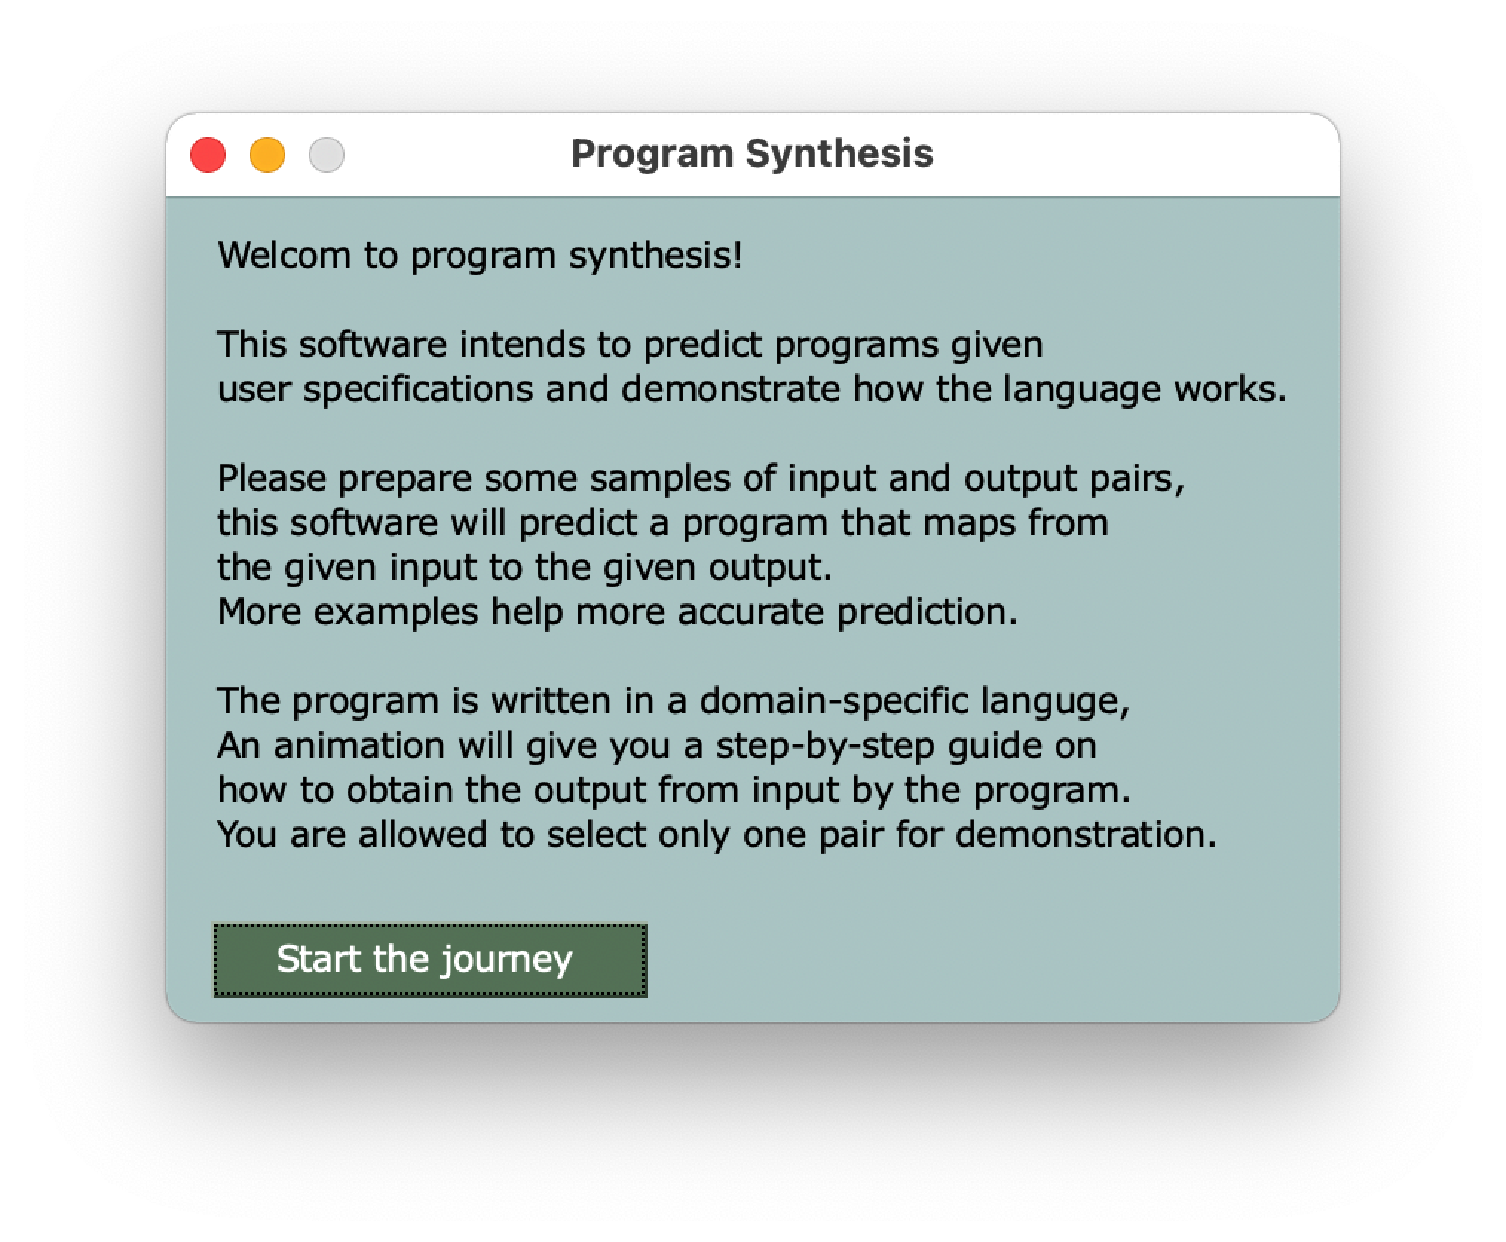
\includegraphics[width=0.55\textwidth]{start.pdf}
	\caption{Main screen}
	\label{fig:main screen}
\end{figure}

The button leads to the window of user specification (Figure \ref{fig:user specification}), you can type the number of input and output pairs that you want to give. These pairs will later be sent to the beam search algorithm to make the prediction and one of them will be selected for demonstration.

\begin{figure}[H]
    \centering
    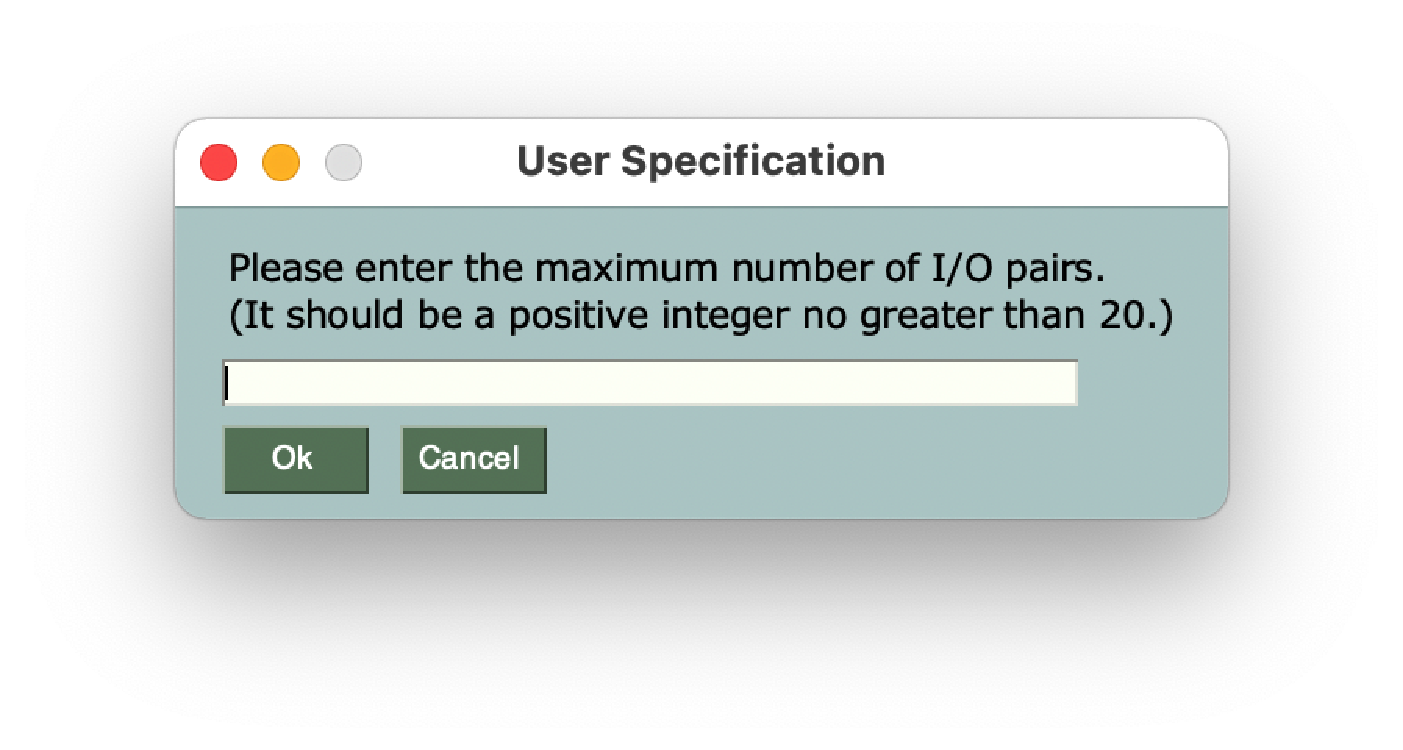
\includegraphics[width=0.55\textwidth]{pairs.pdf}
	\caption{User Specification}
	\label{fig:user specification}
\end{figure}

Then you will be redirected to another window for entering concrete samples. You need to pay attention to the requirements written in the windows box, if you give illegal values, you will get error messages(We will discuss this later in Section \ref{messages}). For example it is six in this case (see Figure \ref{fig:user specification}).

\begin{figure}[H]
    \centering
    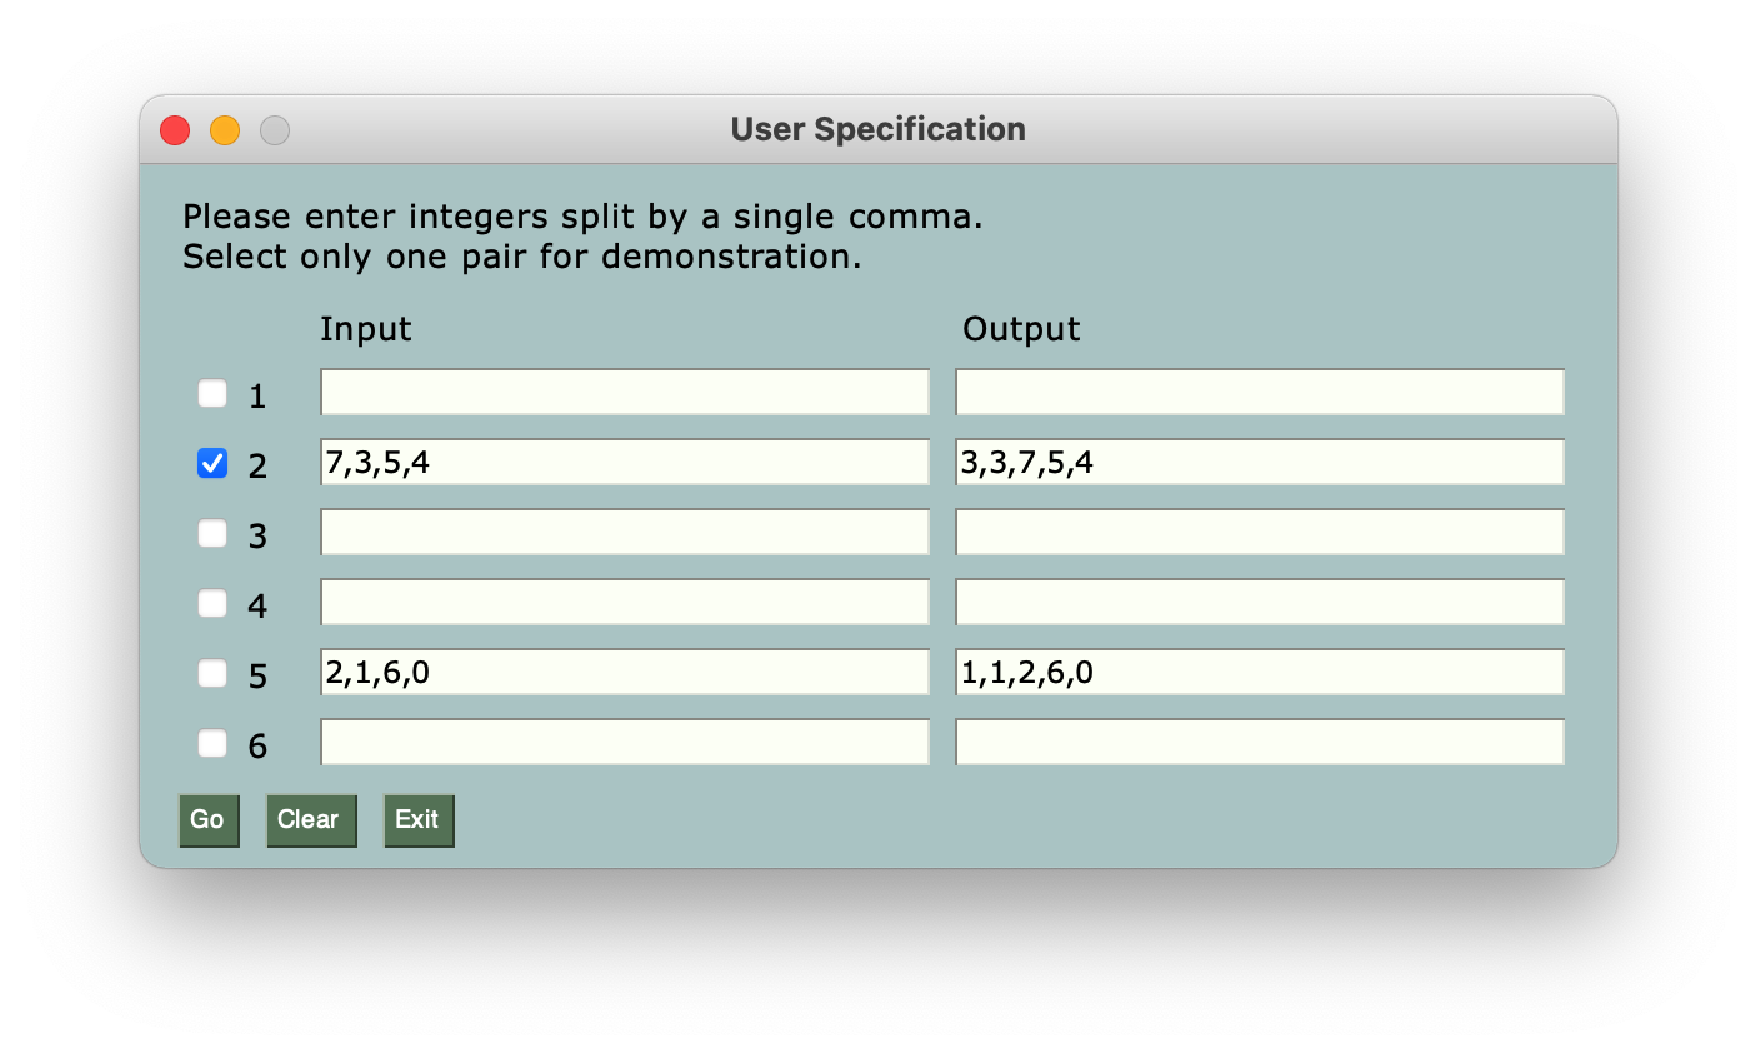
\includegraphics[width=0.6\textwidth]{input.pdf}
	\caption{User Input}
	\label{fig:user input}
\end{figure}

By clicking the ``Ok" button, you will be redirected to another window. Here the user needs to enter at least one pair and at most six pairs of input and output examples. More pairs provide the model with more information, so the result will be more accurate. After finishing the input, you need to choose only one pair among what you have typed for demonstration purpose (as shown in Figure \ref{fig:user input}).
\begin{wrapfigure}{l}{0.45\textwidth}
    \centering
    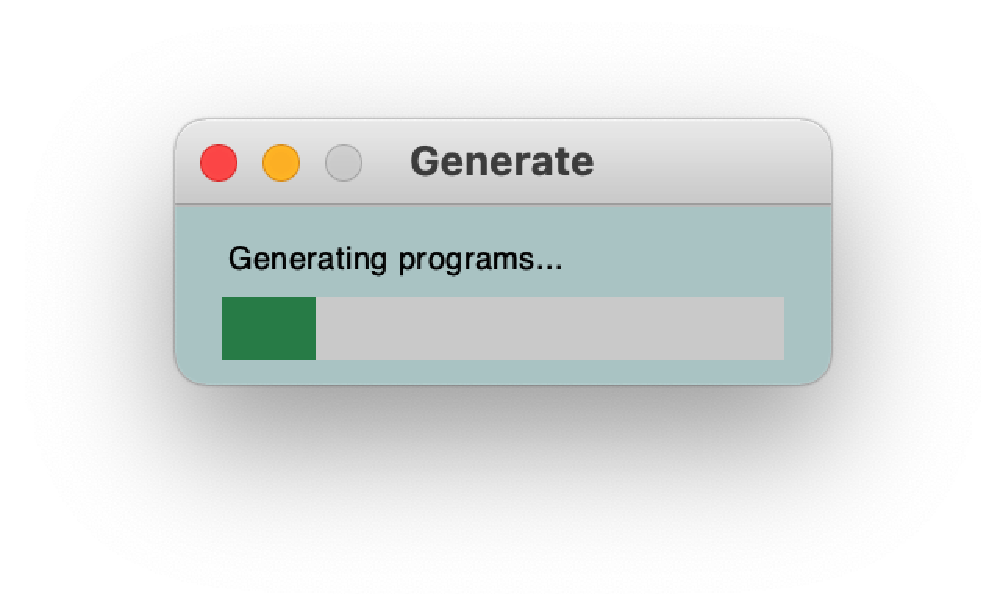
\includegraphics[width=0.4\textwidth]{progress_bar.pdf}
	\caption{Progress Bar}
	\label{fig:progress bar}
\end{wrapfigure}
After specifying all the needed information, the model will work on generating the program to satisfy user input, you will see a screen similar to Figure \ref{fig:progress bar}. The maximum length of the progress bar is set to equal to the max depth of beam search. It is possible that the suitable program is found before the searching reach the deepest level. Therefore, the screen may end before the progress bar reaches the end. 

When beam search gets the desired program, you will the the screen as Figure \ref{fig:demonstrate} shows. On the top of the main screen displays the instructions that can finish the given task. The stack below it starts with the initial state and will change according to the instruction. User can click the ``Next'' button to see how each step works and how the stack changes to go from the input to output with the generated instructions. And the checkbox can be used to hide or show the user input.

\begin{figure}[H]
  \centering
  \begin{minipage}[b]{0.43\textwidth}
    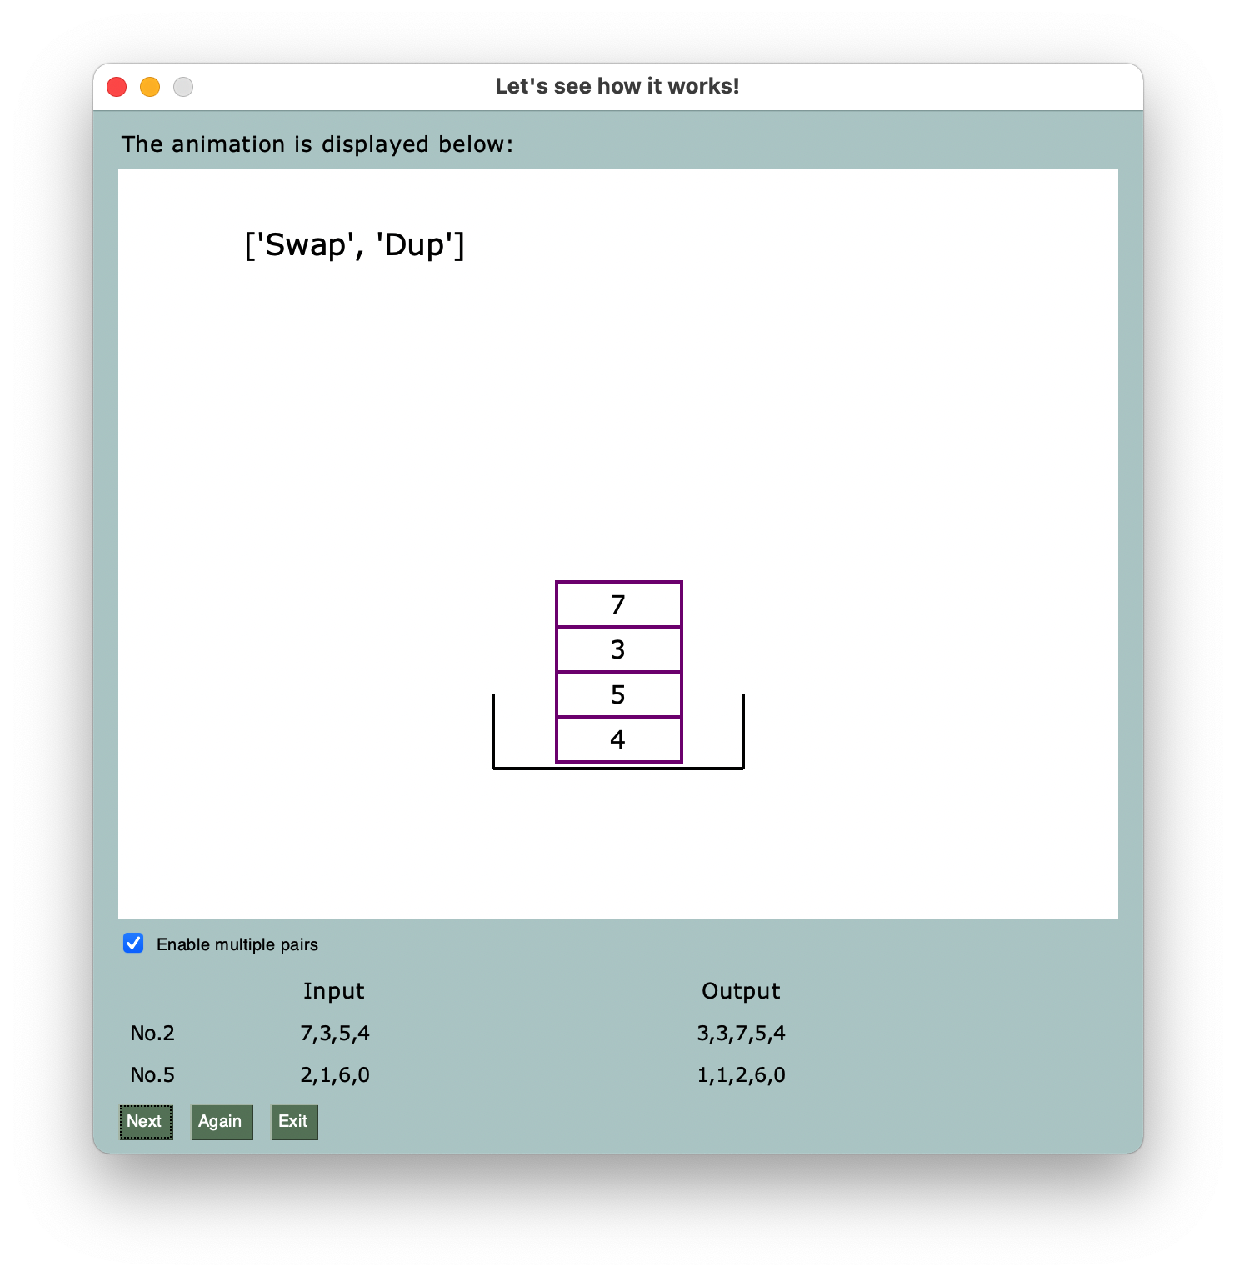
\includegraphics[width=\textwidth]{demonstrate.pdf}
    \caption{Demonstration screen}
    \label{fig:demonstrate}
  \end{minipage}
  \hfill
  \begin{minipage}[b]{0.43\textwidth}
    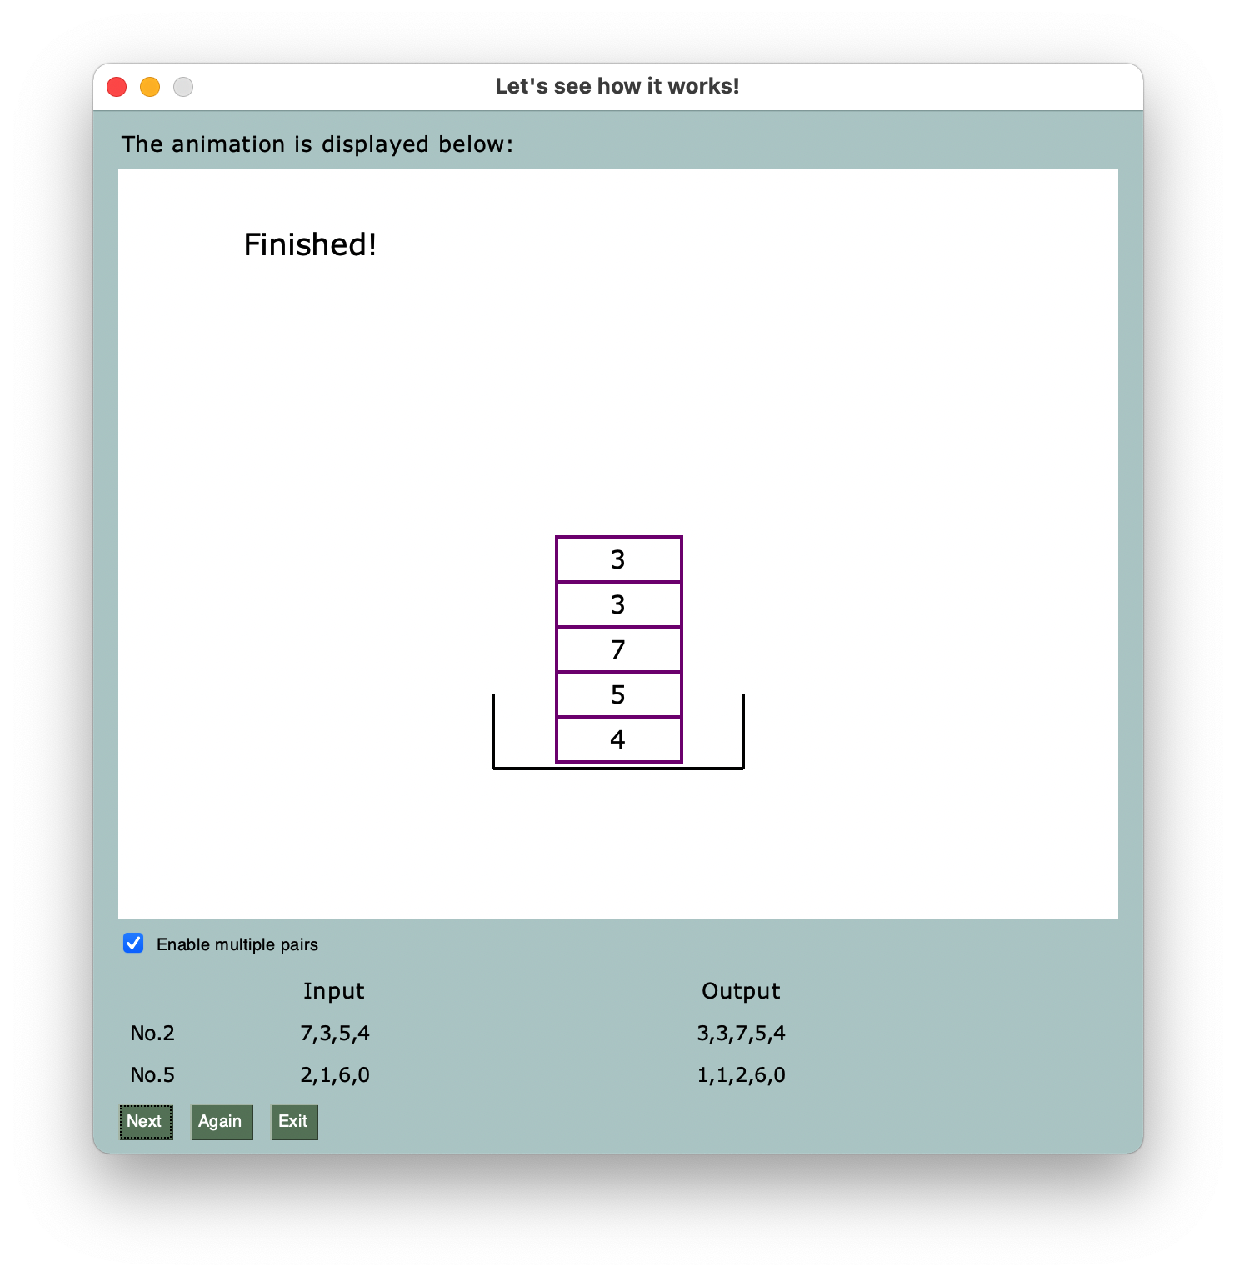
\includegraphics[width=\textwidth]{finish.pdf}
    \caption{Finish screen}
    \label{fig:finish}
  \end{minipage}
\end{figure}

If the search ends, but no program is found, then the user can try again with other input and output pairs.

\subsection{Run-time system messages}
\label{messages}
At the beginning, when the user is required to give a maximum number for input and output pairs, if they press the ``Ok" button without entering an integer or entering other illegal characters which do not meet the requirement of the description, they may get the following error messages.

\begin{figure}[H]
  \centering
  \begin{minipage}[b]{0.28\textwidth}
    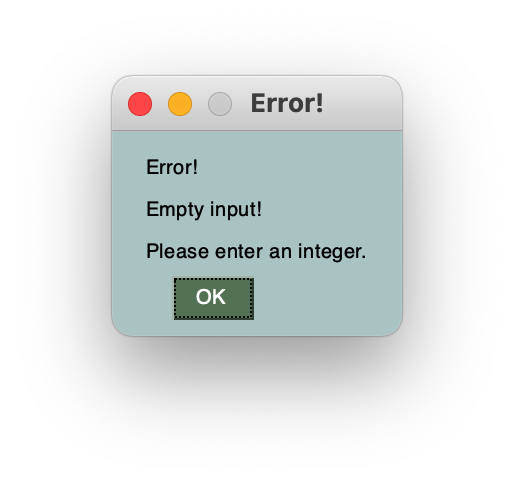
\includegraphics[width=\textwidth]{input_pair_errors/empty_pair.png}
    \caption{Error message for empty input}
  \end{minipage}
  \hfill
  \begin{minipage}[b]{0.29\textwidth}
    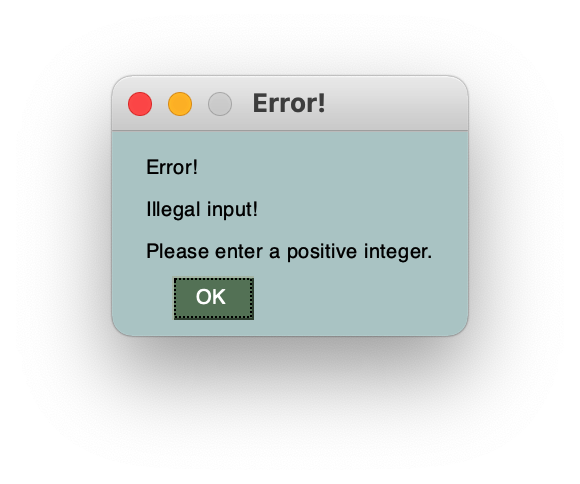
\includegraphics[width=\textwidth]{input_pair_errors/negative_pair.png}
    \caption{Error message for negative numbers}
  \end{minipage}
  \hfill
  \begin{minipage}[b]{0.3\textwidth}
    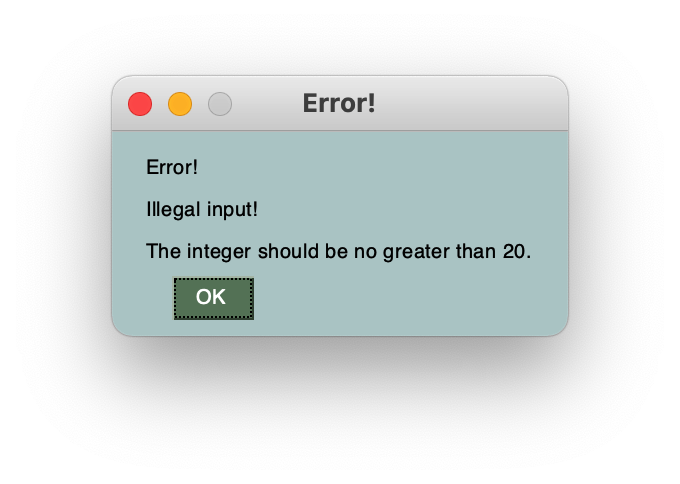
\includegraphics[width=\textwidth]{input_pair_errors/large_pair.png}
    \caption{Error message for large numbers}
  \end{minipage}
\end{figure}

After specifying the custom I/O pairs, the user needs to tick one checkbox for demonstration. They may get the following error messages if:
\begin{itemize}
    \item They forget to select one pair to demonstrate. See Figure \ref{error1}.
    \item They select more than one pair. See Figure \ref{error2}.
\end{itemize}

\begin{figure}[H]
  \centering
  \begin{minipage}[b]{0.4\textwidth}
    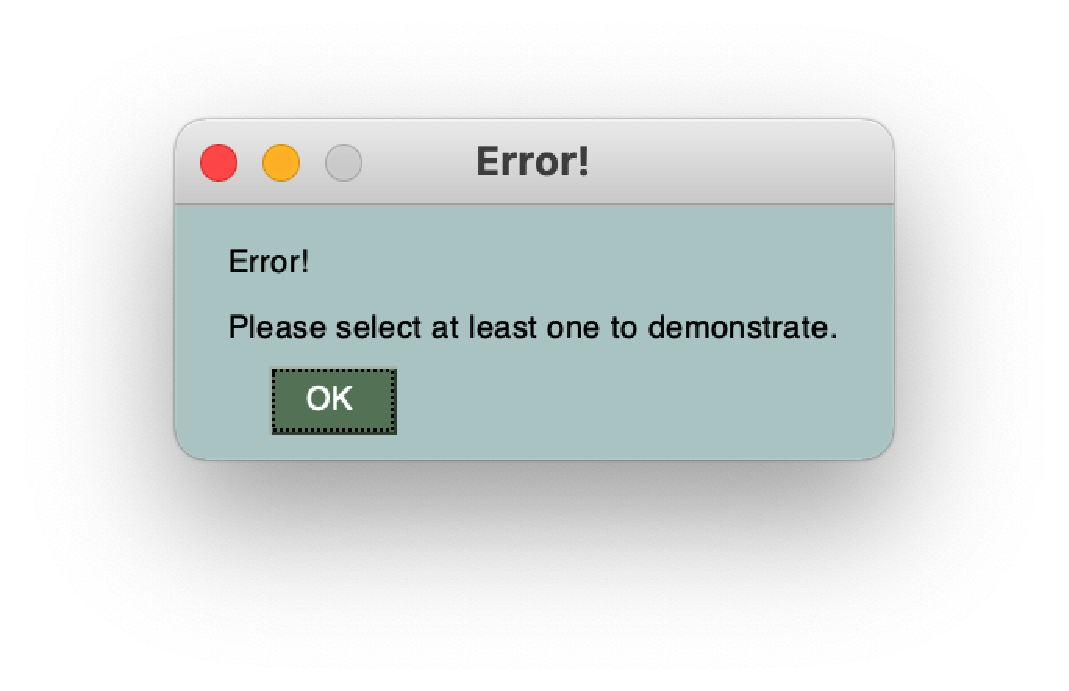
\includegraphics[width=\textwidth]{error1.pdf}
    \caption{Error message for not selecting}
    \label{error1}
  \end{minipage}
  \hfill
  \begin{minipage}[b]{0.4\textwidth}
    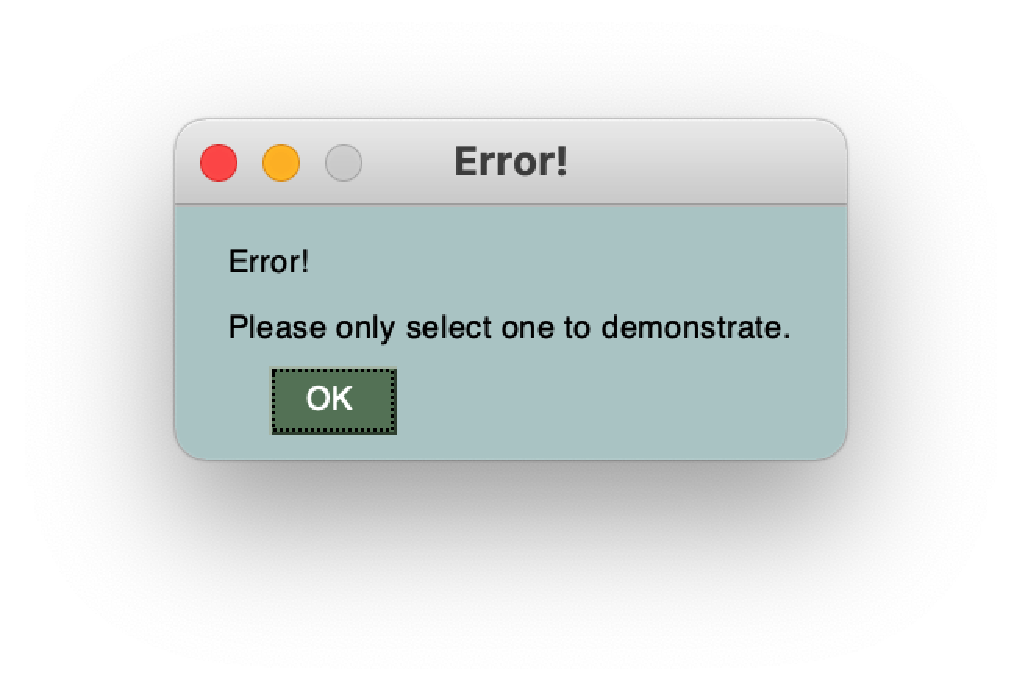
\includegraphics[width=\textwidth]{error2.pdf}
    \caption{Error message for multiple selecting}
    \label{error2}
  \end{minipage}
\end{figure}